% Sections/02_dataset.tex
% Dataset and Processing Section

\section{Dataset and Processing}
\label{sec:dataset}

The UCI Human Activity Recognition data set has 10,299 samples from 30 participants(clients) performing 6 activities (WALKING, WALKING\_UPSTAIRS, WALKING\_DOWNSTAIRS, SITTING, STANDING, LAYING)~\cite{anguita2013public}. The sample includes 561 normalized features derived from accelerometer and gyroscope sensors, having values adjusted in the range [-1.000, 1.000] with zero missing values.

The counts reveal an excellent equilibrium in between LAYING (1,944 samples, 18.9\%) and STANDING (1,906 samples, 18.5\%) being the most populated classes, whereas the remaining activities range from 1,406-1,777 samples (13.7\%-17.3\%). The distribution of the subjects is quite uniform with each subject contributing 300-400 samples (mean=343 and median=342), thereby offering well-balanced federated learning environments.

\subsection{Preprocessing Pipeline}
\label{subsec:preprocessing}

The loading process of the dataset involves automated integrity checks affirming the full 10,299 $\times$ 561 feature matrix over 6 activity classes with extensive data quality validation. All 561 features are min-max scaled to the range of [-1.000, 1.000], which guarantees equalized feature scales and avoids high-value sensor readings dominating during model training.

Data is divided by subject IDs, forming 30 standalone federated clients where every client holds one subject's full activity profile. This federation by subjects reflects actual situations when individual user data is stored on personal devices alone~\cite{mcmahan2017communication}.

\begin{figure}[htbp]
  \centering
  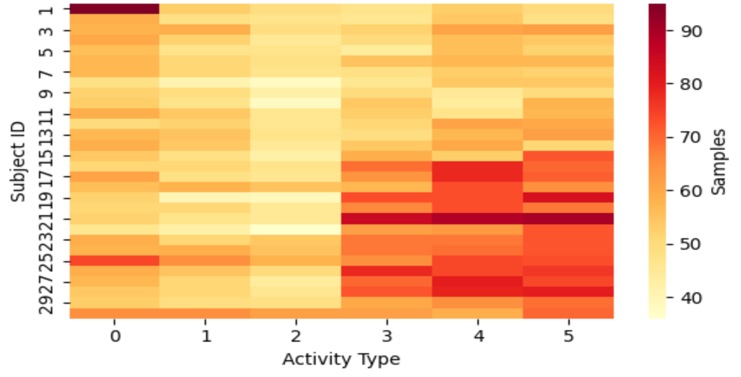
\includegraphics[width=0.7\textwidth]{figures/fig2.png}
  \caption{Subject-Activity matrix shows distribution of activity sample across 30 subjects in the dataset}
  \label{fig:subject_activity}
\end{figure}

Correlation analysis of the first 30 features shows organized relationships between the sensor measurements, with variance analysis selecting the most informative 20 features (variance range: 0.090-0.142), with enough variability for successful learning. The preprocessing workflow ensures data integrity by systematic validation, load-balanced client distribution, and variance optimization of features, providing high-quality input for federated learning experiments.
